\documentclass{article}

% if you need to pass options to natbib, use, e.g.:
% \PassOptionsToPackage{numbers, compress}{natbib}
% before loading nips_2016
%
% to avoid loading the natbib package, add option nonatbib:
% \usepackage[nonatbib]{nips_2016}

% \usepackage{nips_2016}

% to compile a camera-ready version, add the [final] option, e.g.:
\usepackage[final]{midway-report}

\usepackage[utf8]{inputenc} % allow utf-8 input
\usepackage[T1]{fontenc}    % use 8-bit T1 fonts
\usepackage{hyperref}       % hyperlinks
\usepackage{url}            % simple URL typesetting
\usepackage{booktabs}       % professional-quality tables
\usepackage{amsfonts}       % blackboard math symbols
\usepackage{nicefrac}       % compact symbols for 1/2, etc.
\usepackage{microtype}      % microtypography
\usepackage{graphicx}
\usepackage{float}

\title{10-703 Project: Midway Report}

\author{Kumail Jaffer \And Sidhanth Mohanty \And Phillip
Wang
\AND
\texttt{mjaffer@andrew.cmu.edu} \And
\texttt{smohant1@andrew.cmu.edu}\And
\texttt{pkwang@andrew.cmu.edu}}

\begin{document}

\maketitle

\section{Introduction}
The goal of this project is to try out novel ideas for
solving multiagent cooperative games, as well as try
ideas and variants from current literature.

Our project direction has deviated significantly from the
initial project proposal. We still draw many ideas from
Hierarchical Reinforcement Learning, but have switched because
we found this problem more motivated and interesting.

We set up a cooperative game to capture salient features
of the multiagent reinforcement learning setting.
The game is set up in the following way: there is a target
$q_t$ at some location in the box $[-1,1]\times[-1,1]$
and there are 3 agents $q_1,q_2,q_3$ at points in the circle of
radius $\sqrt{2}$ around the origin. The agents can move
in one of 8 directions at a certain speed (all angles
$\frac{2\pi i}{8}$ for $i=0,1,\ldots,7$) and exert a force
on the target, which induces motion. The goal is to
keep the target inside the box for as long as possible.
The agents are confined to the unit circle of radius
$\sqrt{2}$ around the origin $B(0,\sqrt{2})$.
The force that an agent exerts on the target is $\frac{C}{r^2}$
where $r$ is the distance between the agent and target, and
the target accelerates at a rate proportional to the force.
For each timestep that the target stays in the box, the
environment gives a reward of value 1.

The state is given by the following information: position and velocity
of the target, and position and velocity of each agent $i$.

In a single time step, the state changes in the following way:
the positions of the target and agent are updated based on
current velocity, the target's velocity is updated
based on the acceleration induced by the forces
of agents, calculated based on current positions. Then the
velocities of the agents are calculated based on the
actions of the agents.

The inherent trouble with using standard approaches of treating
the ensemble of agents as a single agent is that the action
space then suffers from the curse of dimensionality, which
calls for a large number of training iterations to
learn. Another fairly intuitive approach might be to
train each agent separately on the environment, but
this fails to capture the notion that the actions of
different agents need to be coherently coordinated,
and each agent taking actions individually may not
result in coordinated actions.

In order to have coordination between agents while
simultaneously keeping the dimensionality
of the action space small, we use techniques inspired
by the literature of hierarchical reinforcement learning,
and multiagent reinforcement learning: specifically in
the setting where the agents are collaborating.
The papers and their contributions are sketched in
the `Literature Survey' section below, and our exact
approach to the problem is described in more depth
in the `Methods' section.

\subsection*{Literature Survey}

In recent years, there has been a lot of hype in Deep
Reinforcement Learning \cite{mnih2015human}, achieving
human-level performance in complex domains such as Atari
\cite{mnih2013playing} and Go \cite{silver2016mastering}. At
the same time, there is extensive work in Multiagent
Reinforcement Learning \cite{busoniu2008comprehensive},
especially in the context of robotics \cite{spaan2002high,
 fox2000probabilistic, mataric1997reinforcement}. More recently,
work has been done in marrying the two ideas, such as
\cite{tampuu2017multiagent}, which examines cooperative
and competitive multiagent behavior in Pong with Deep Q-networks by
tampering with environment rewards, or
\cite{usunier2016episodic, peng2017multiagent}, which applies multiagent deep
reinforcement learning on StarCraft micromanagement tasks.


Some research has been done on multiagent reinforcement learning
with limited communication. DIAL (Differentiable Inter-agent Learning) \cite{foerster2016learning},
is an approach in which
each agent acts as an independent learner, and agents communicate
by passing messages. In particular, each agent is modeled by
a Recurrent Neural Network that outputs an action and a message
to be passed to each subsequent agent. During test time, these
agents can only communicate through a channel with limited bandwidth.
On the other hand, CommNet \cite{sukhbaatar2016learning}, which
has a single controller for actions and communication
between the agents, also performs well in situations where each agent only
observes parts of the environment. Researchers at OpenAI
have developed ways to learn grounded compositional language
\cite{mordatch2017emergence} by letting multiple agents
communicate only over limited differentiable channels.


Our approach for multiagent collaboration draws inspiration from
Hierarchical Reinforcement Learning \cite{kulkarni2016hierarchical}. These techniques are used to learn
temporal abstraction by learning a metacontroller, which picks
a subtasks, and a subcontroller, which learns to perform each
subtask well. The idea is: when going from one place to another,
one doesn't think about each step he/she takes, but rather
thinks in terms of composing subtasks that he/she knows how to do (go to
the bus stop, take the bus, walk down three blocks, etc.).
These techniques have been used to solve environments with
sparse rewards like Montezuma's Revenge and Minecraft
\cite{tessler2016deep}.

\section{Methods}

To solve this problem, we have four different methods, with the
first two being the baseline that uses approaches we learned
from class in a straightforward manner, and the other two being
more sophisticated so they can beat the baseline. The
reason we implemented the first two methods is to
convince ourselves that
this problem indeed calls for more involved techniques.


\subsection{Method 1: single agent DQN}
Our first method is a straightforward application of
DQNs to this
problem where we treat the three agents as a single agent,
where the action is given by a 3D vector, with the
entries being the action of the corresponding agents.
The problem with this approach and the reason we don't expect
this approach to work well is that the number of actions blows
up to $9^3=729$ and hence the resulting high sample complexity
of the problem would require a large number of training
iterations to converge.

We follow the DQN approach of \cite{mnih2013playing}
where the state $S$ of the game is given as input to a
neural network and the output of the neural network
is a vector of $Q$-values of dimension equal to the
size of the action space, where the $i$th entry of the
vector corresponds to the estimate of $Q(S,a_i)$ where $a_i$
is the $i$th action. The action taken is then decided
based on the vector of $Q$-values using methods like
a $\varepsilon$-greedy policy.

The exact architecture of the neural network is
a fully connected layer with ReLU activation
with output dimension 20, followed by
a linear layer with output dimension
equal to the total number of actions.

To train this DQN (called the online network), we also maintain
a target DQN that we train against. We first start the game
by playing a number of random actions and as
more time steps pass, we anneal the
probability of picking a random action down,
store tuples of
$\texttt{(state, action, reward, next state)}$
in an experience buffer (for using experience
replay while training), and every few iterations,
train the neural net on a batch of 32 randomly
sampled examples from the replay buffer. And
for some $T$, the target network's weights
are updated to those of the online network every
$T$ steps.

We implemented this and the results are described in
the `Results' section.

\subsection{Method 2: a DQN per agent}
A natural step to try next to combat the blow-up
of the action space is to treat each agent
individually. There are three $Q$ functions:
$Q_1, Q_2$ and $Q_3$, one for each agent, and
for each state-action pair $\langle S,a\rangle$,
there are estimates $Q_1(S,a),Q_2(S,a)$ and
$Q_3(S,a)$. We train three DQNs in a way similar
to what was described in the previous section
(using target fixing and experience replay), one for
each $Q_i$.

The architecture of the each DQN is the same as the
previous method, except instead of having an output
layer of dimension $729$, the output layer has dimension
just $9$. When in state $S$, agent $i$ selects which one
of 9 actions to pick based on an $\varepsilon$-greedy policy
on the $Q$-values $Q(S,a)$.

Since this greatly decreases the dimensionality of
the action space, we expect the convergence to be
faster: however we don't expect this technique to
converge to a good policy because our setup
of training as well as actions taken by each agent
fails to capture the notion of coordination or
communication needed between agents to play effectively.

We ran experiments for this, and described the results in
the `Results' section.

\subsection{Method 3: Conditional DQN}
This is a modification of \textbf{Method 2} to incorporate
the notion of coodination and somehow have agents communicate
with each other, drawing ideas from \cite{foerster2016learning}.

We describe the neural network architecture that we train
on.
\begin{itemize}

\item The input to the first layer is the state vector of
the game: the first layer is a fully connected layer
with 20 output units with activation ReLU.

\item The second layer is a fully connected linear layer
with 9+9 output units: the first nine correspond to the $Q$-values
of the 9 actions for input state $S$ for agent 1: call
this $q_1$, and the next 9 correspond to a `message' $h_1$ that
we intend on passing to later agents.

\item The next layer takes in $h_1$ as well as input
state vector $S$ and has activation ReLU and 20 output
units.

\item Then there is a fully connected linear layer with
9+9 output units, which correspond to the $Q$-values
of the 9 actions for input state $S$ for agent 2
along, called $q_2$, along with a message $h_2$
for agent 3.

\item A fully ReLU layer takes in $h_2$ and the input
state $S$ and has 20 output units.

\item The 20 output units from the previous layer are
passed in through a fully connected linear layer with
9 output units to obtain the $Q$-values for the 9
possible actions for agent 3 based on the current state
and the $Q$-value estimates of agent 1 and agent 2
to get vector $q_3$.

\item The output of the neural net is $\langle q_1,q_2,q_3
\rangle$.

\end{itemize}

The actions are selected for agent $i$ using $q_i$,
presumably using $\varepsilon$-greedy.
The vector $h_i$ highlights the entries with
high $Q$-values and intuitively captures
what agent $i$ might do, and it's expected that
passing along this information intuitively helps
with coordination. The training routine is the same as that
of a standard DQN (using randomly sampled examples from
a replay buffer and a target that is fixed).
Following the setups from \cite{foerster2016learning,
sukhbaatar2016learning}, the three neural networks share
weights.


\subsection{Method 4: Hierarchical Multiagent Approach}
Inspired by the use of the metacontroller-subcontroller
hierarchy for temporal abstraction in \cite{kulkarni2016hierarchical}, we try a similar approach
to achieve coordination between multiple agents in an
environment where the metacontroller plays the role of the `coordinator' by delegating
tasks to the agents. The way the agents make their moves is via a subcontroller,
which learns to obey the directions given to it by the metacontroller

The metacontroller learns to output target
impulses, where the $i$th target impulse is the total impulse
that agent $i$ has on the target, equal to the momentum
imparted by agent $i$ on the target. The change in momentum of the target due to
agent $i$ in the time interval $(t_1,t_2)$ is given by
\[
\Delta p = \int_{t_1}^{t_2} F_i(t)dt
\]
where $F_i(t)$ is the force exerted by agent $i$ on the target at time $t$.

The metacontroller gives a goal impulse that an agent tries to inflict on the target
for a period of 100 timesteps. Let $(\Delta p)_i$ be the impulse of the agent
on the target so far at timestep $i$. Define $\Phi_i$ as $\|(\Delta p)_i - L\|_2$ at timestep $i$.
The reward to the subcontroller guiding the agent at timestep $i$ woud be
$\Phi_{i-1}-\Phi_i$, thus giving a positive reward for making the total impulse
closer to the target.

The subcontroller takes in a state and the goal and outputs $Q$-values, based on which
an action is taken via a $\varepsilon$-greedy policy, and the way the subcontroller is
trained would be the way a DQN is trained, like in the previous methods.

The goal given by the metacontroller can be viewed as it's action. Since the action
space is continuous, standard techniques of estimating the $Q$-values of every action
are not well-defined any more. Fortunately, \cite{lillicrap2015continuous} resolves
this using actor-critic methods to deterministically select a continuous action
given a state. The setup involves an actor network that ouputs a continuous state based
on an input state, and this is trained using a critic network, which approximates the
value of input states on actions given by the actor network. The rewards to the metacontroller
are the cumulative rewards of the environment over the 100 steps where the subcontroller
took steps based on the goals given to it.


\section{Preliminary Results}

So far, we've implemented the toy environment we described, as well as methods
1 and 2, and run them on an instance of the environment with three agents.

Method 1 fails to converge to any sort of reasonable policy. This was expected,
since the size of our action space is enormous if we treat the three agents as a
single agent. As visible in figure 1, the losses continuously decrease and never
begin increasing. This is probably because the model is so complex, it takes a
long time to train. As visible in figure 2, the average reward of the agent
increases over time, though it never does anything amazing, and never reaches
the performance of a human player.
Videos of the agent seem to begin to learn a meaningful
strategy, but it takes the agent a lot of time.

\begin{figure}[H]
\centering
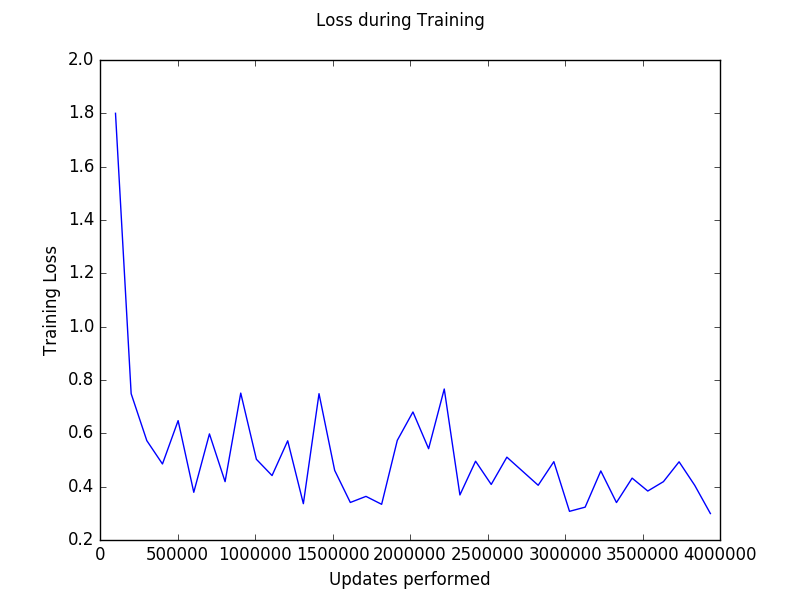
\includegraphics[scale=0.5]{dqn-training-loss}
\caption{Losses during training for method 1}
\end{figure}

\begin{figure}[H]
\centering
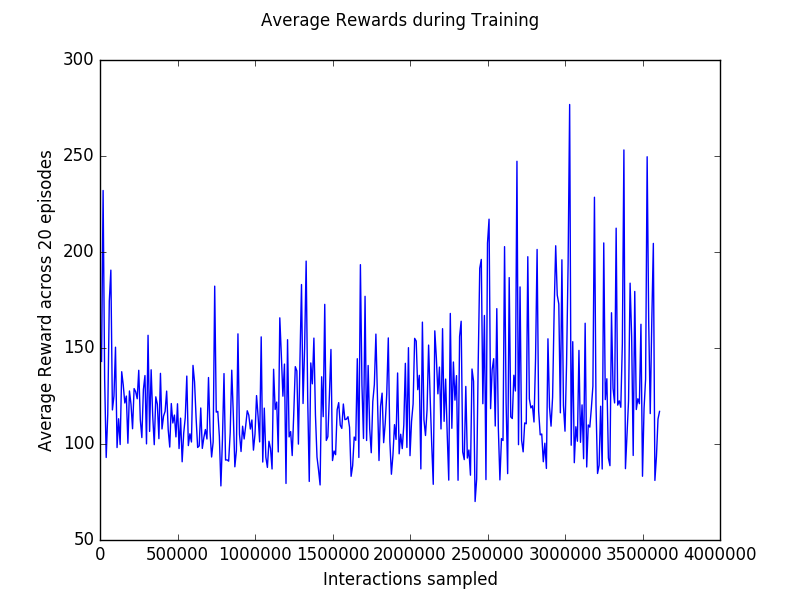
\includegraphics[scale=0.5]{dqn-average-reward}
\caption{Average rewards during training for method 1}
\end{figure}

Method 2 is a little more promising. The losses decrease until some inflection
point, where they begin increasing, as you would expect (if they never
increased, one might be concerned that the model is overfitting). The average
rewards seem to roughly increase over time, and the best policy this learns is
better than that of model 1. The model learned, however, is quite
unstable. With a gap of only a few hundred training updates, the policy the
network learns can go from wildly successful to wildly unsuccessful. We suspect
this may be because this model doesn't coordinate the actions of the agents very
well, and hope that the other two models can help to do this.

\begin{figure}[H]
\centering
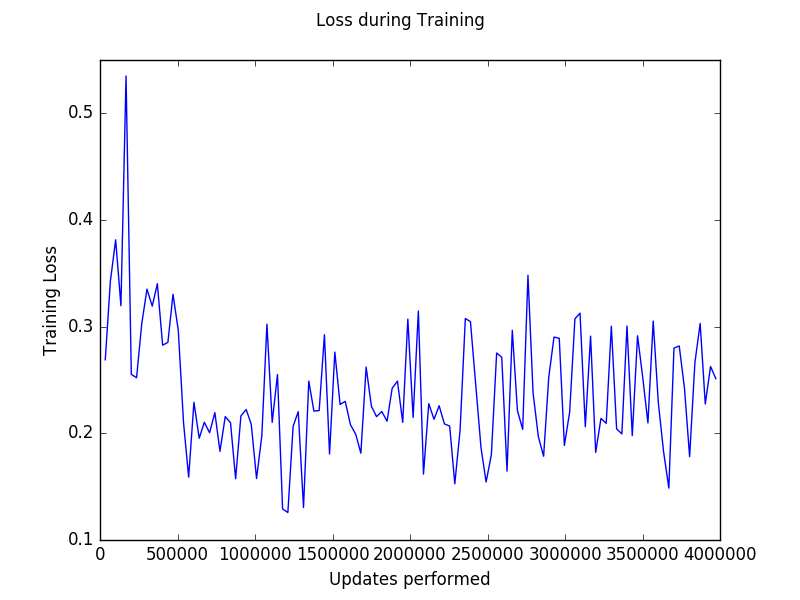
\includegraphics[scale=0.5]{dqn-multi-training-loss}
\caption{Average rewards over time for method 2}
\end{figure}

\begin{figure}[H]
\centering
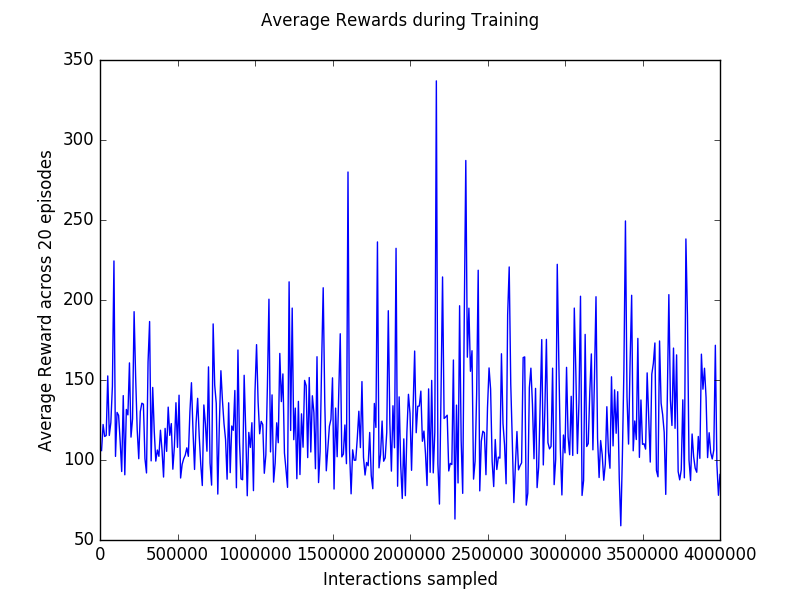
\includegraphics[scale=0.5]{dqn-multi-average-reward}
\caption{Average rewards during training for method 2}
\end{figure}

The visibibility of the trends in these graphs is slightly complicated by the
fact that the agent's success is extremely sensitive to the starting position.
There are some positions from which it is extremely difficult to get a good
score. This means that the agent's performance necessarily has high variance and
its average reward gets obscured.

To get a sense of what the agent learns, it is helpful to look at videos of the
strategies it learns. We provide them here:
\url{https://www.youtube.com/playlist?list=PL2Hlc8GXcnpfXdMdBUpE0rjldxPwK2ZxR}

\section{Final Plan}
We plan to get a running implementation of Method 3 and Method 4, with the goal
of having it beat the benchmarks that we implemented using Method 1 and Method 2.
We also intend to implement the current state-of-the-art methods
in multiagent reinforcement learning \cite{foerster2016learning, sukhbaatar2016learning, peng2017multiagent},
and compare their results to method 4.

Other extensions to the project would include adding more agents, making the agents heterogeneous,
(e.g. varying the magnitude of charge that agents carry), and increasing the speed at which
some agents may move. Another extension would be to implement the environment with partial
information, where each agent knows their own position and velocity and only positions of other
agents, and compare how the four methods fare against eachother.

\bibliographystyle{plain}
\bibliography{midway-report}

% \section*{References}

% References follow the acknowledgments. Use unnumbered first-level
% heading for the references. Any choice of citation style is acceptable
% as long as you are consistent. It is permissible to reduce the font
% size to \verb+small+ (9 point) when listing the references. {\bf
%   Remember that you can use a ninth page as long as it contains
%   \emph{only} cited references.}
% \medskip

% \small

% [1] Alexander, J.A.\ \& Mozer, M.C.\ (1995) Template-based algorithms
% for connectionist rule extraction. In G.\ Tesauro, D.S.\ Touretzky and
% T.K.\ Leen (eds.), {\it Advances in Neural Information Processing
%   Systems 7}, pp.\ 609--616. Cambridge, MA: MIT Press.

% [2] Bower, J.M.\ \& Beeman, D.\ (1995) {\it The Book of GENESIS:
%   Exploring Realistic Neural Models with the GEneral NEural SImulation
%   System.}  New York: TELOS/Springer--Verlag.

% [3] Hasselmo, M.E., Schnell, E.\ \& Barkai, E.\ (1995) Dynamics of
% learning and recall at excitatory recurrent synapses and cholinergic
% modulation in rat hippocampal region CA3. {\it Journal of
%   Neuroscience} {\bf 15}(7):5249-5262.

\end{document}
